\ProvidesFile{chapters/ch-Top_Quark_Physics.tex}

\chapter{TOP QUARK PHYSICS AT THE LHC}
\label{Top_Quark_Physics_at_the_LHC}
The top quark was predicted in 1973 by Kobayashi and Maskawa when the Cabibbo matrix was extended to the CKM matrix~\cite{10.1143/PTP.49.652} in order to accommodate the experimental discovery of CP-violation in precision measurements of kaon regeneration~\cite{PhysRevLett.13.138}.
This extension necessarily required three quark generations, when at the time only the up, down, and strange quarks were known.
The charm quark was discovered in 1974~\cite{PhysRevLett.33.1404},\cite{PhysRevLett.33.1406} and the bottom quark in 1977~\cite{PhysRevLett.39.252}.
After searching for two decades, the top quark was finally discovered in 1995 at Fermi National Acceleration Laboratory (FNAL), jointly by the CDF~\cite{PhysRevLett.74.2626} and D0~\cite{PhysRevLett.74.2632} Tevatron Experiments.
It is the heaviest elementary particle ever discovered, with a measured mass $m_t = 172.69 \pm 0.30 \; \si{\GeV}$~\cite{bib:PDG}, the top quark has a mass equivalent to a Tungsten isotope containing 184 nucleons; it is \sim$35$ times heavier than the next heaviest quark, the bottom quark, as illustrated in figure~\ref{QuarkMasses}.
\begin{figure}[htb]
  \begin{center}
    \begin{tabular}{c}
        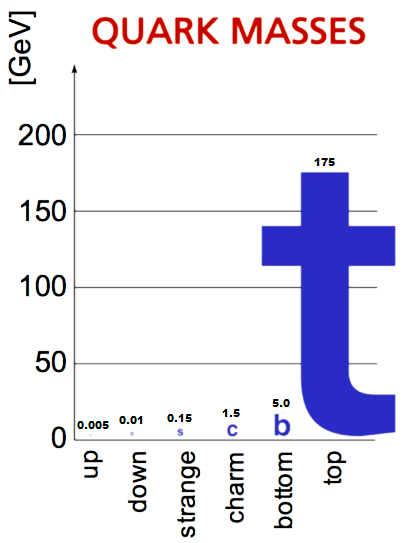
\includegraphics[width=0.325\textwidth]{fig_TopQuark/TopQuarkMass.png}
        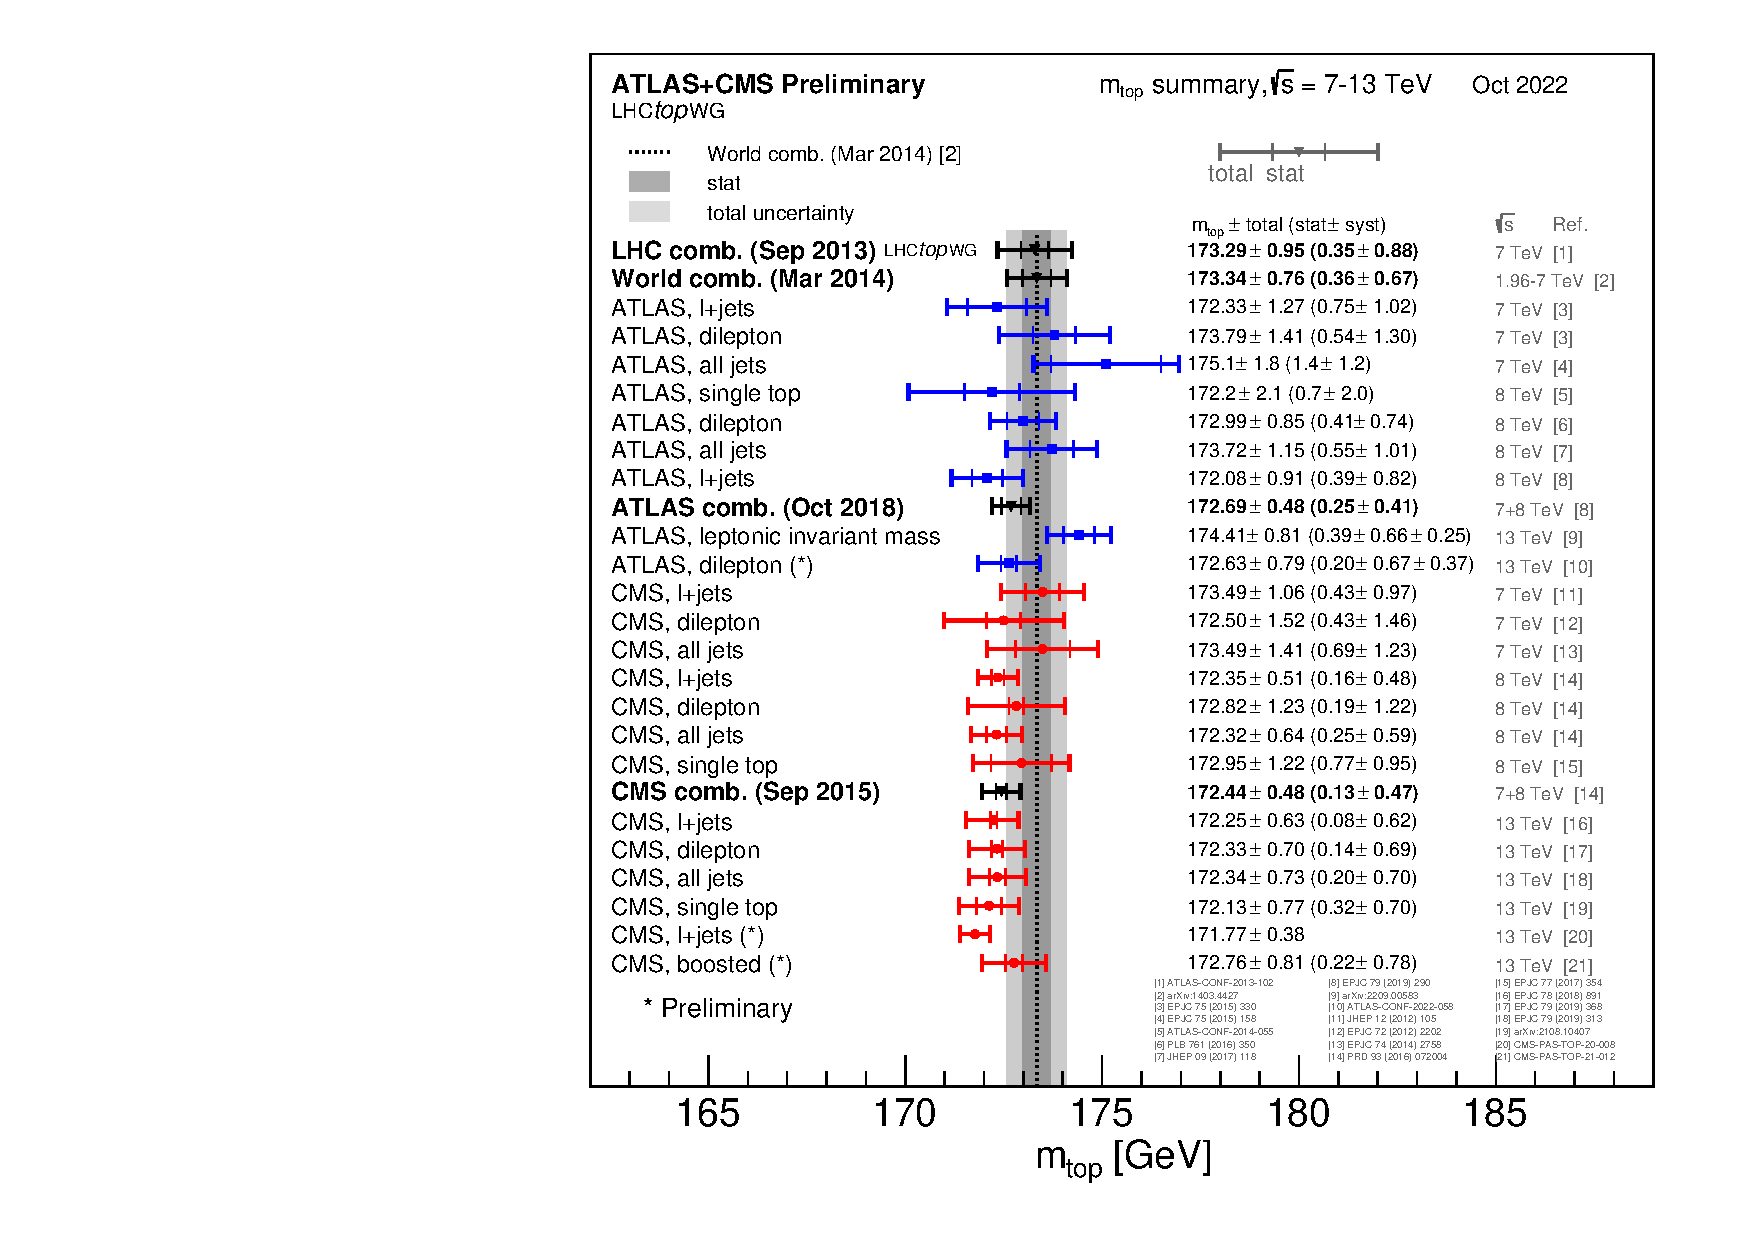
\includegraphics[width=0.45\textwidth]{fig_TopQuark/LHC_topmass_oct22.pdf}
    \end{tabular}
    \caption{The top quark is the heaviest elementary particle ever discovered and is \sim$35$ times heavier than the next heaviest quark (Left).
            Summary of the ATLAS and CMS direct measurements of top quark mass (Right)~\cite{LHCTopWGSummaryPlots}.
            }
    \label{QuarkMasses}
  \end{center}
\end{figure}
Due to its very large mass, the top quark has a very short lifetime, or equivalently, a large decay width.
The top quark full decay width is larger than the QCD hadronization scale and much larger than the spin decorrelation scale.
Thus, not only do top quarks decay before hadronizing\footnote{Theoretical predictions for toponium bound state production at the \beamenergy LHC are around 0.8\% the total \ttbar production cross-section~\cite{PhysRevD.104.034023}.  Experimental evidence for toponium production has not yet been observed.} to form bound states but also their properties, including spin information, are transferred to their decay products.
The spin information of top quarks is observable in the angular kinematic distributions of their decay products.
These properties make top quarks unique in the quark sector, as top quark measurements are the only opportunity to study the properties of bare quarks, free of QCD confinement and hadronization effects.

\section{Top Quark Pair Production}
\label{Top_Quark_Pair_Production}
Because of the large mass, the production of top quarks has only been possible by Tevatron and LHC high-energy accelerator experiments.
At these colliders, the majority of top quarks are produced in \ttbar pairs by the strong interaction, but single $t$ production by the electroweak interaction is also possible.
For \ttbar production, three parton production processes are possible at hadron colliders: gluon-gluon ($gg$) fusion, quark/anti-quark ($q\bar{q}$) annihilation, and quark-gluon scattering.
While at the Tevatron $q\bar{q}$ annihilation was the dominant production mechanism, for \beamenergy proton-proton collisions at the LHC, the gluon density of the proton parton distribution function (PDF) is much higher than the quark density (see section~\ref{sec:Parton_Distribution_Functions}), and $gg$ fusion accounts for \sim$90 \%$ of \ttbar production.

The inclusive \ttbar production cross-section in proton-proton ($pp$) collisions is calculated by convoluting the proton PDFs with the partonic cross-sections and summing over all parton constituents of the proton, i.e. gluons, valence quarks, and sea quarks.
For QCD \ttbar production, three channels of LO $gg$ fusion and one channel of LO $q\bar{q}$ annihilation parton production processes are possible.
LO Feynman diagrams for these processes are shown in figure~\ref{ttbar_production_LO_feynman_diagrams}.
\begin{figure}[htb]
  \begin{center}
    \begin{tabular}{cccc}
        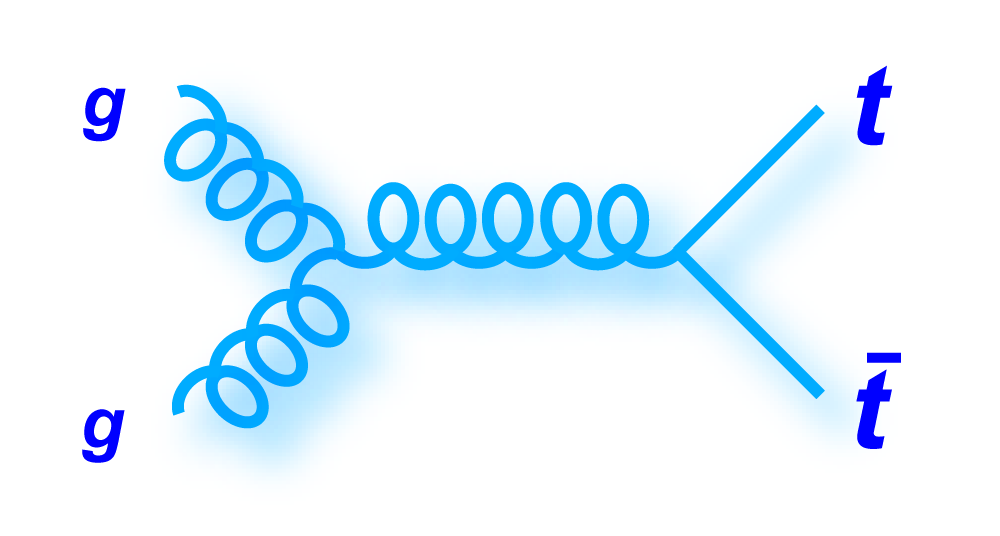
\includegraphics[width=0.245\textwidth]{fig_TopQuark/feynman_ttbar_LHC_gggtt.png}
        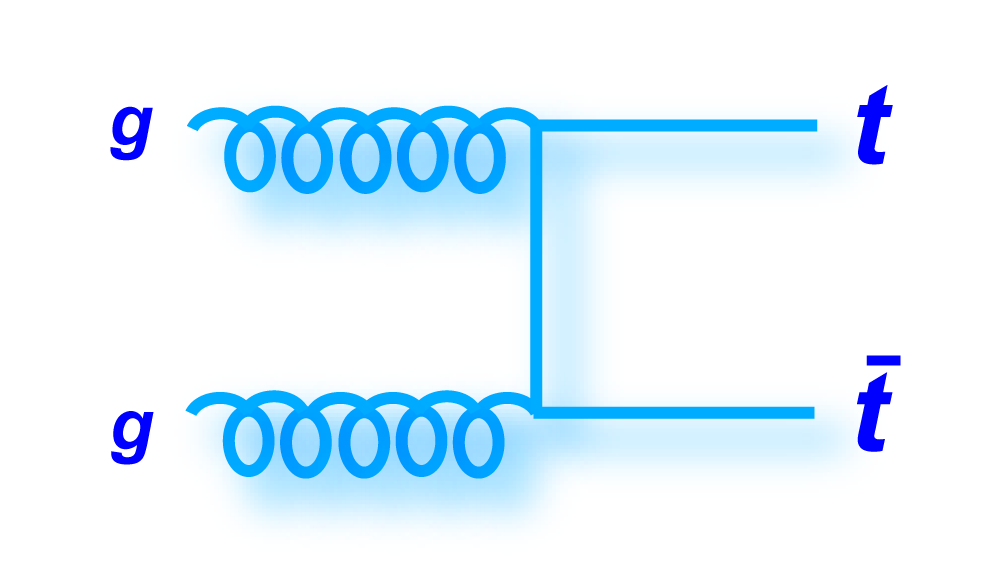
\includegraphics[width=0.245\textwidth]{fig_TopQuark/feynman_ttbar_LHC_ggttt.png}
        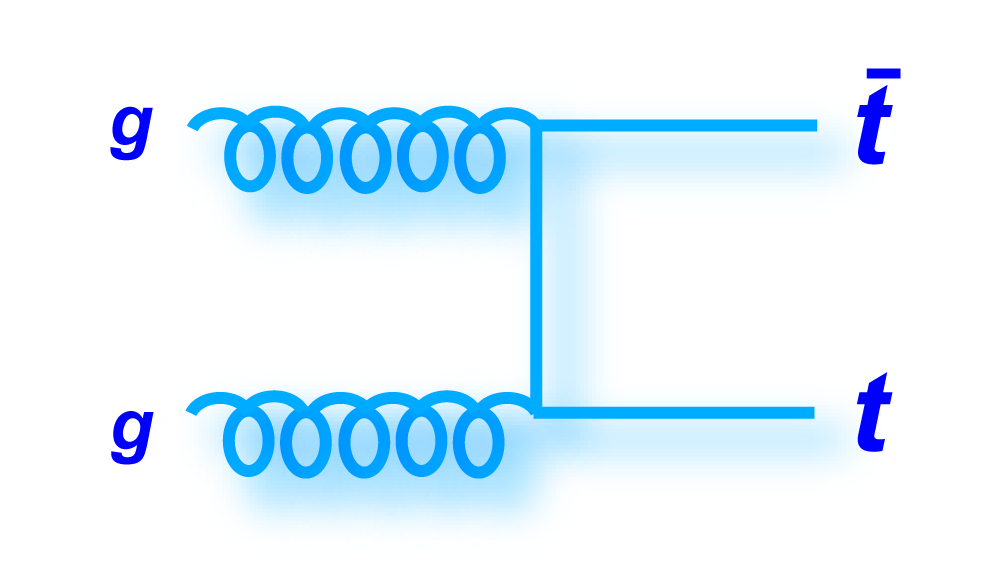
\includegraphics[width=0.245\textwidth]{fig_TopQuark/feynman_ttbar_LHC_ggttbart.png}
        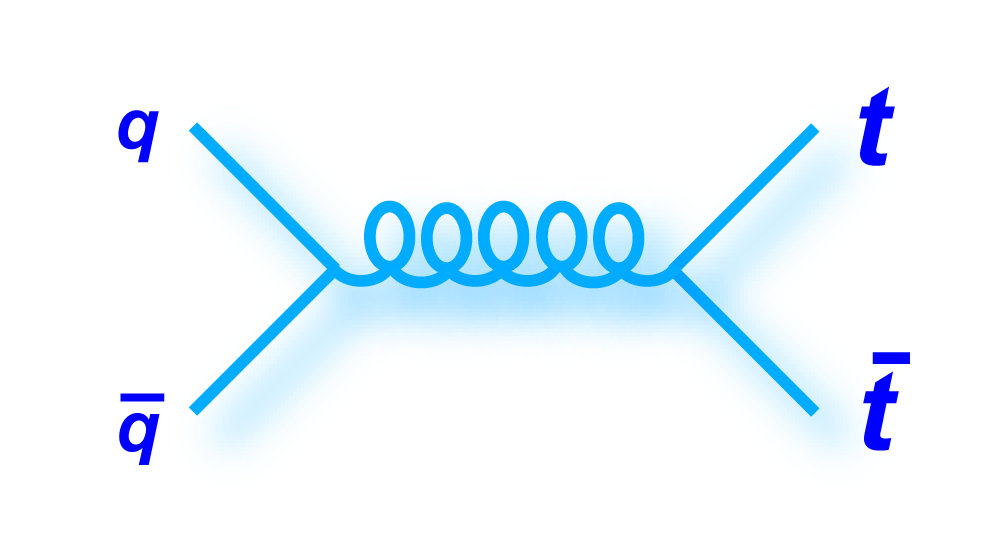
\includegraphics[width=0.245\textwidth]{fig_TopQuark/feynman_ttbar_LHC_qqgtt.png}
    \end{tabular}
    \caption{LO Feynman diagrams for QCD \ttbar production: three channels of $gg$ fusion and one channel of $q\bar{q}$ annihilation~\cite{d0_diagrams}.
            }
    \label{ttbar_production_LO_feynman_diagrams}
  \end{center}
\end{figure}
Quark-gluon scattering can also produce \ttbar pairs, but only at NLO and higher orders.
At next-to-next-to-leading-order (NNLO) with next-to-next-to-leading-logarithmic (NNLL) precision for \beamenergy, assuming $m_t = \SI{172.5}{\GeV}$, the inclusive \ttbar production cross-section is calculated to be $\sigma_{\ttbar} = 831.76 \substack{+19.77 \\ -29.20} \; (\text{Scale}) \; \pm 35.06 \; (\text{PDF} + \alpha_S) \; \si{\pico \b}$.
A summary of \ttbar cross-section measurements by LHC and Tevatron experiments as a function of the center-of-mass energy, as well as a summary of \ttbar cross-section measurements by ATLAS and CMS at \beamenergy are shown in figure~\ref{ttbar_cross-section}.
\begin{figure}[htb]
  \begin{center}
    \begin{tabular}{cc}
        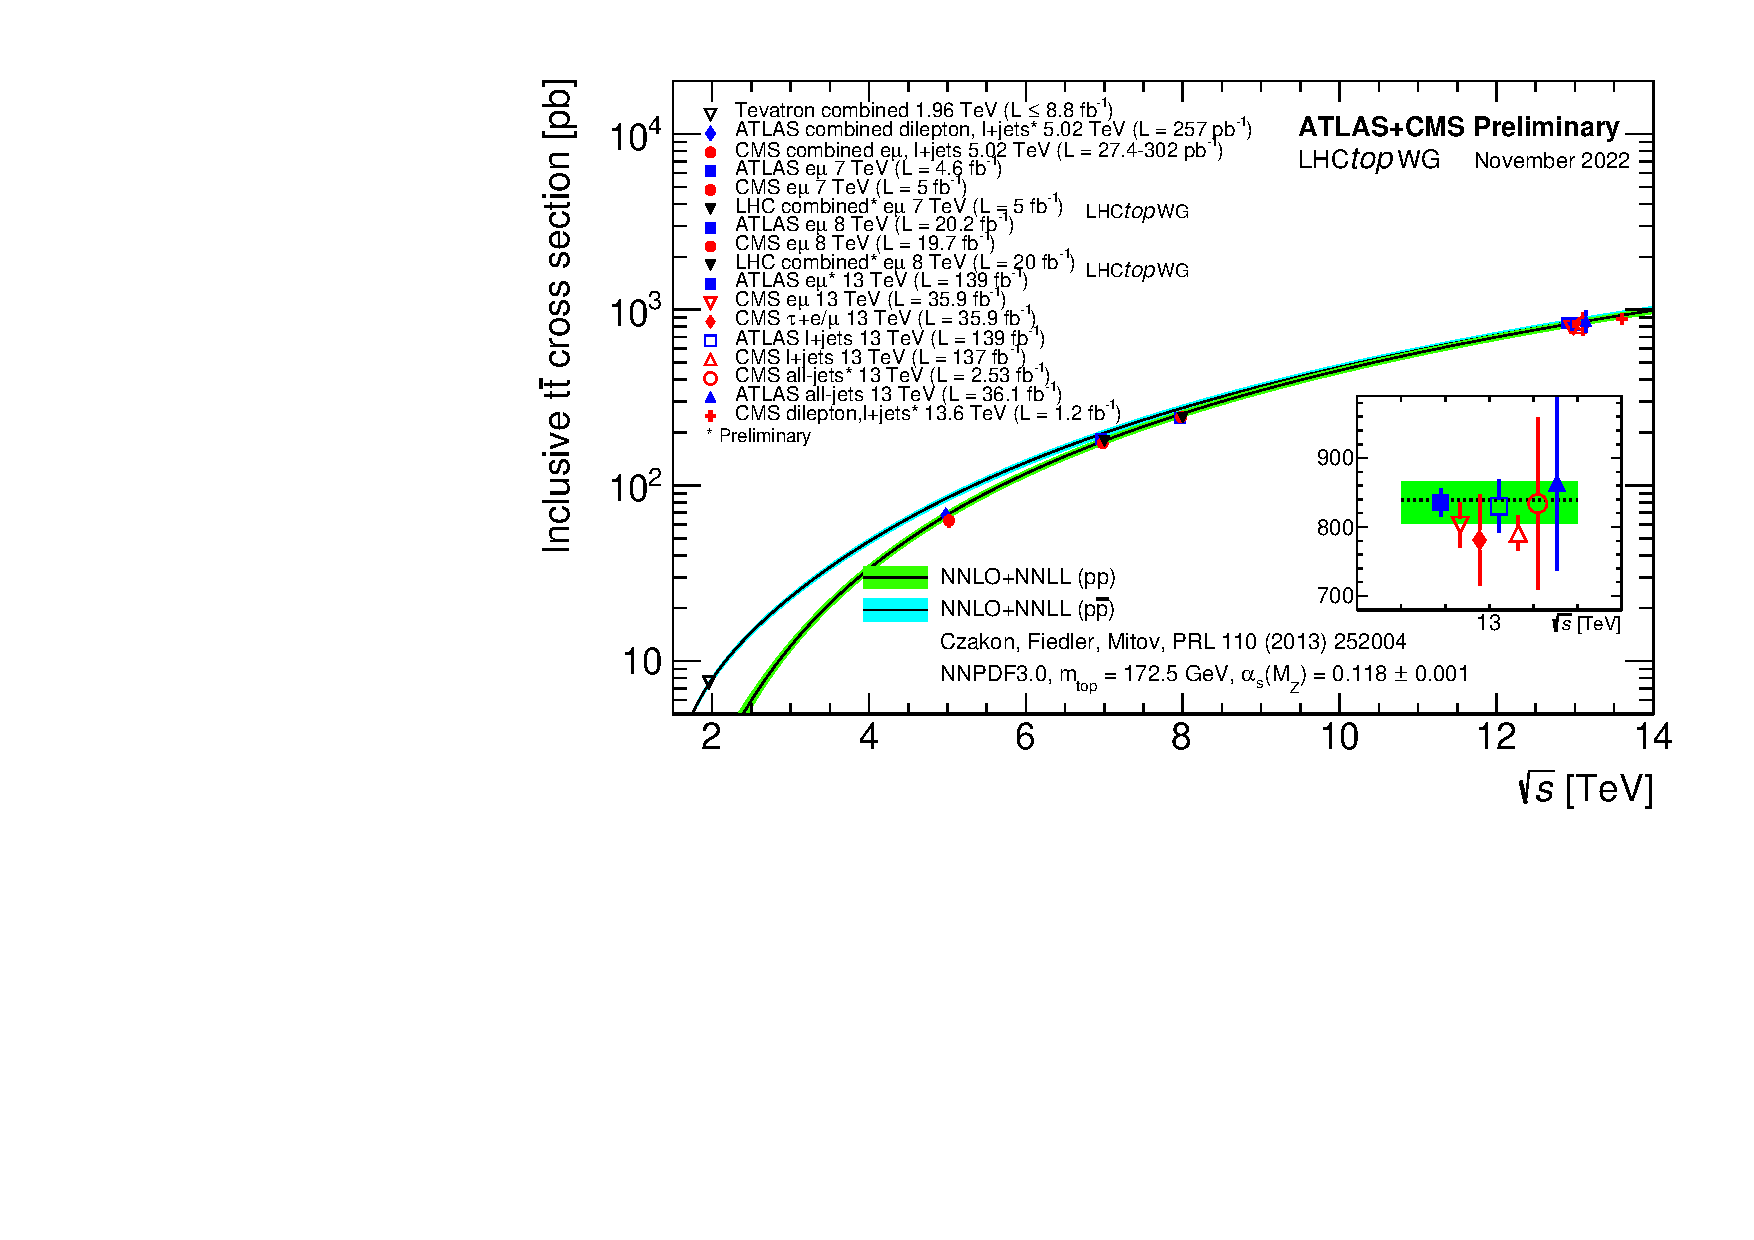
\includegraphics[width=0.60\textwidth]{fig_TopQuark/tt_curve_toplhcwg_nov22.pdf}
        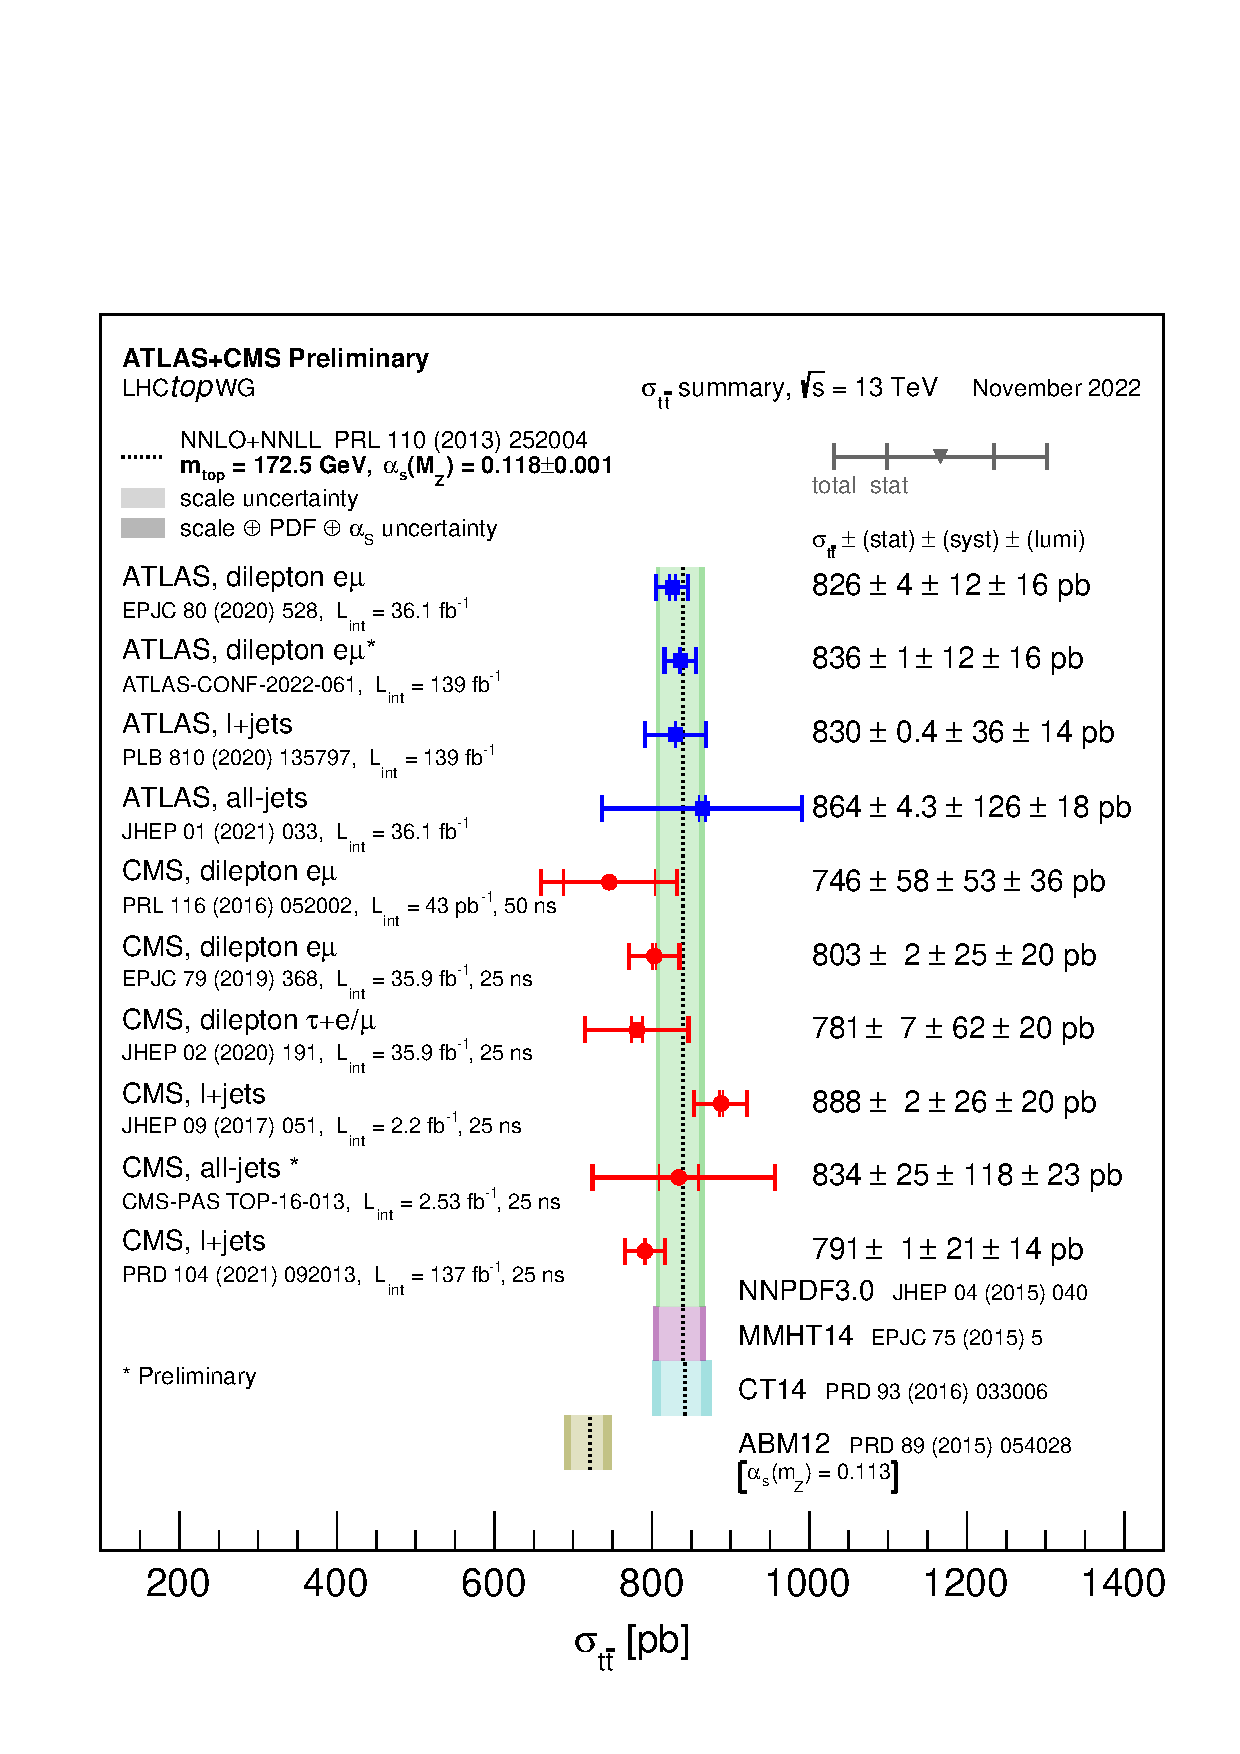
\includegraphics[width=0.35\textwidth]{fig_TopQuark/tt_xsec_13TeV_nov22.pdf}
    \end{tabular}
    \caption{Summary of LHC and Tevatron measurements of the top-pair production cross-section as a function of the center-of-mass energy compared to the NNLO QCD calculation complemented with NNLL resummation (Left).
    Summary of measurements of the top-pair production cross-section at \beamenergy compared to the exact NNLO QCD calculation complemented with NNLL resummation (Right)~\cite{LHCTopWGSummaryPlots}.
            }
    \label{ttbar_cross-section}
  \end{center}
\end{figure}

\section{Decays of Top Quark Pairs}
\label{Decays_of_Top_Quark_Pairs}
The top quark decay width $\Gamma_t$ implies a lifetime of $\tau_t = \sfrac{1}{\Gamma_t}=\SI{4.6e-25}{\s}$ before decaying via the weak interaction into an on-shell $W$-boson and down-type quark ($t \rightarrow W^+ q$).
The branching ratio of each mode can be calculated using elements of the CKM matrix $B_x = \frac{\vert V_{tx} \vert^2}{\vert V_{tb} \vert^2 + \vert V_{ts} \vert^2 + \vert V_{td} \vert^2}$, and while any of the down-type quarks are possible, because $\vert V_{tb} \vert = 0.999118 \; >> \; \vert V_{ts} \vert = 0.04110 \; \text{or} \; \vert V_{td} \vert = 0.00857$~\cite{bib:PDG}, $t \rightarrow W^+ b$ dominates with a branching ratio $ B_b \simeq 99.8\%$.

The $W$-boson can decay hadronically $W^+ \rightarrow q \bar{q^\prime}$, where $q$ is an up-type quark ($u$ or $c$) and $\bar{q^\prime}$ is an anti-down-type quark ($\bar{d}$, $\bar{s}$, or $\bar{b}$), or leptonically $W^+ \rightarrow \bar{\ell} \nu_\ell$, where $\bar{\ell}$ is an anti-lepton ($\bar{e}$, $\bar{\mu}$, or $\bar{\tau}$) and $\nu_\ell$ is a neutrino of the same lepton flavor~\ref{t_decay}.
\begin{figure}[htb]
  \begin{center}
    \begin{tabular}{cc}
        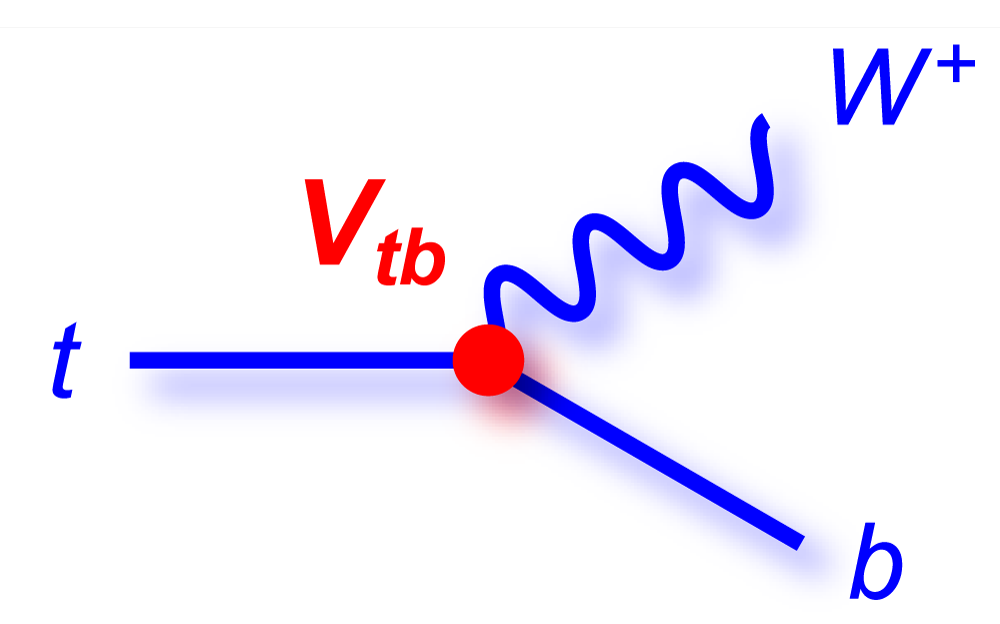
\includegraphics[width=0.45\textwidth]{fig_TopQuark/feynman_t_decay_Vtb_blue.png}
        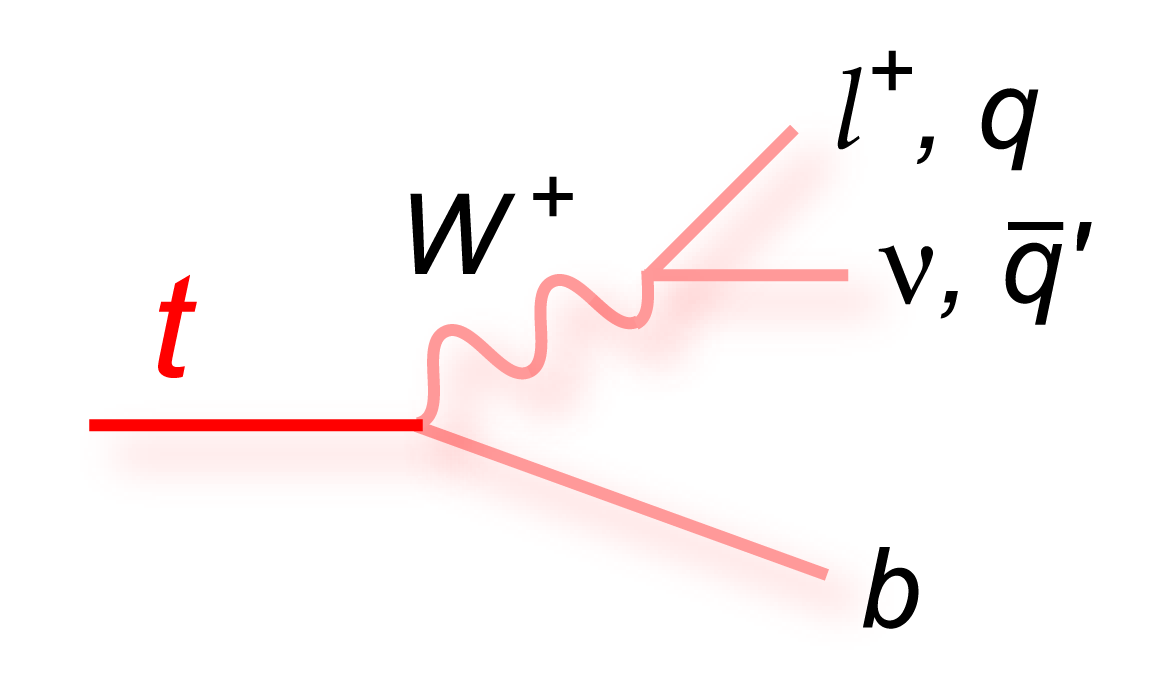
\includegraphics[width=0.45\textwidth]{fig_TopQuark/feynman_t_decay_ljetsqq_pink.png}
    \end{tabular}
    \caption{The branching modes of $t \rightarrow W^+ q$ depend on the values of CKM matrix elements (Left).
             The $W$-boson can decay hadronically or leptonically (Right)~\cite{d0_diagrams}.
    }
    \label{t_decay}
  \end{center}
\end{figure}
Ignoring phase space considerations, the relative branching fractions of the hadronic and leptonic decay modes are given by the ratio of flavor combinations and color combinations, together with the corresponding squared CKM matrix elements:
\begin{linenomath*}
{\small
\begin{align}
\frac{\text { hadronic }}{\text { leptonic }}=\frac{ \{ u\bar{d}:{\vert V_{ud} \vert}^2, u\bar{s}:{\vert V_{us} \vert}^2, u\bar{b}:{\vert V_{ub} \vert}^2, c\bar{d}:{\vert V_{cd} \vert}^2, c\bar{s}:{\vert V_{cs} \vert}^2, c\bar{b}:{\vert V_{cb} \vert}^2 \} \times \{ R, B, G\} }{ \{ e \bar{\nu_e }, \mu \bar{\nu_\mu}, \tau \bar{\nu_\tau} \}} = \frac{6}{3}
\end{align}
}%
\end{linenomath*}
where decays with top quarks are forbidden due to energy conservation, and due to the unitary of the CKM matrix ${\vert V_{ud} \vert}^2 + {\vert V_{us} \vert}^2 + {\vert V_{ub} \vert}^2 = {\vert V_{cd} \vert}^2 + {\vert V_{cs} \vert}^2 + {\vert V_{cb} \vert}^2 = 1$.
Including phase space considerations, the hadronic $W$-boson decay mode occurs $(66.5 \pm  1.4) \%$ of the time, and the leptonic mode occurs $(33.2 \pm 1.0) \%$~\cite{bib:PDG}.

For a \ttbar pair, depending on the $W$-boson decays of the $t$ and $\bar{t}$, there are three decay modes: 
\begin{itemize}
    \item {\bf Fully Hadronic:} $t\bar{t} \rightarrow W^+ b \; W^- \bar{b} \rightarrow q \bar{q^\prime} b \; \bar{q^{\prime\prime}}  q^{\prime\prime\prime} \bar{b}$, also referred to as ``all jets''
    \item {\bf Semi-Leptonic:} $t\bar{t} \rightarrow W^+ b \; W^- \bar{b} \rightarrow  q \bar{q^\prime} b \; \ell \bar{\nu_{\ell}} \bar{b} $ or $t\bar{t} \rightarrow W^+ b \; W^- \bar{b} \rightarrow  \bar{\ell} \nu_\ell b \; \bar{q^{\prime\prime}}  q^{\prime\prime\prime} \bar{b}$, also referred to as ``lepton + jets''
    \item {\bf Dileptonic:} $t\bar{t} \rightarrow W^+ b \; W^- \bar{b} \rightarrow \bar{\ell} \nu_\ell b \; \ell^{\prime} \bar{\nu_{\ell^{\prime}}} \bar{b}$
\end{itemize}
Examples of LO Feynman diagrams for the \ttbar decay modes are shown in figure~\ref{Top_Pair_Decay_FeynmanDiagrams}.
\begin{figure}[htb]
  \begin{center}
    \begin{tabular}{c}
        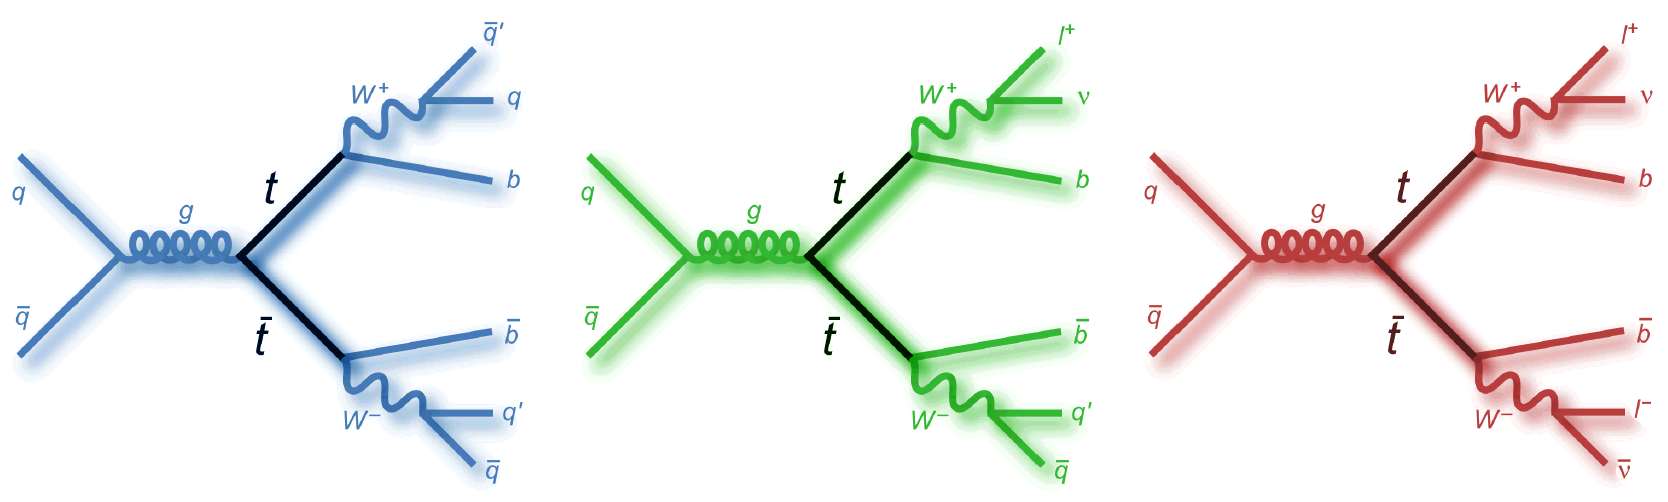
\includegraphics[width=0.99\textwidth]{fig_TopQuark/ttbar_decay_feynman_diagrams.png}
    \end{tabular}
    \caption{Examples of LO Feynman diagrams for the \ttbar decay modes: Fully Hadronic (Left), Semi-Leptonic (Middle), and Dileptonic (Right)~\cite{d0_diagrams}
            }
    \label{Top_Pair_Decay_FeynmanDiagrams}
  \end{center}
\end{figure}
Because hadronic $W$-boson decay modes are more common than leptonic ones, for \ttbar decays the dileptonic mode occurs least often \sim$10.5 \%$~\cite{bib:PDG}.
A schematic classifying \ttbar decay modes, together with a chart showing the relative branching fractions, is shown in figure~\ref{Top_Pair_Decay_Channels}.
\begin{figure}[htb]
  \begin{center}
    \begin{tabular}{cc}
        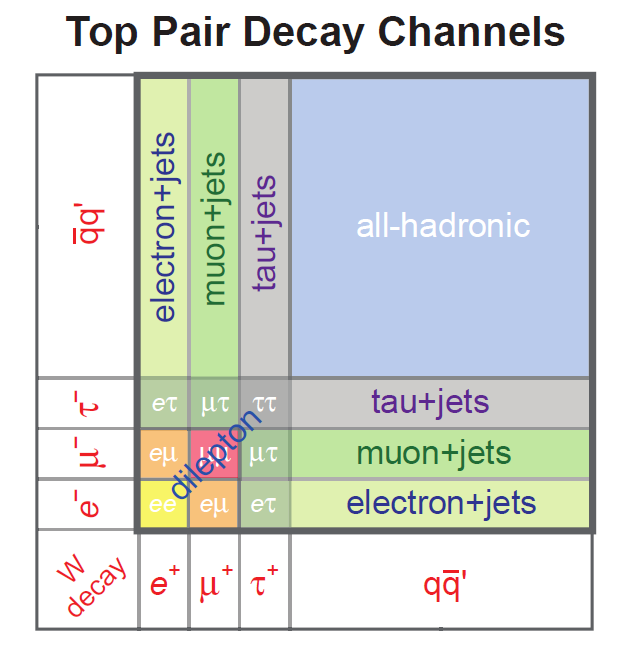
\includegraphics[width=0.45\textwidth]{fig_TopQuark/Top_Pair_Decay_Channels.png}
        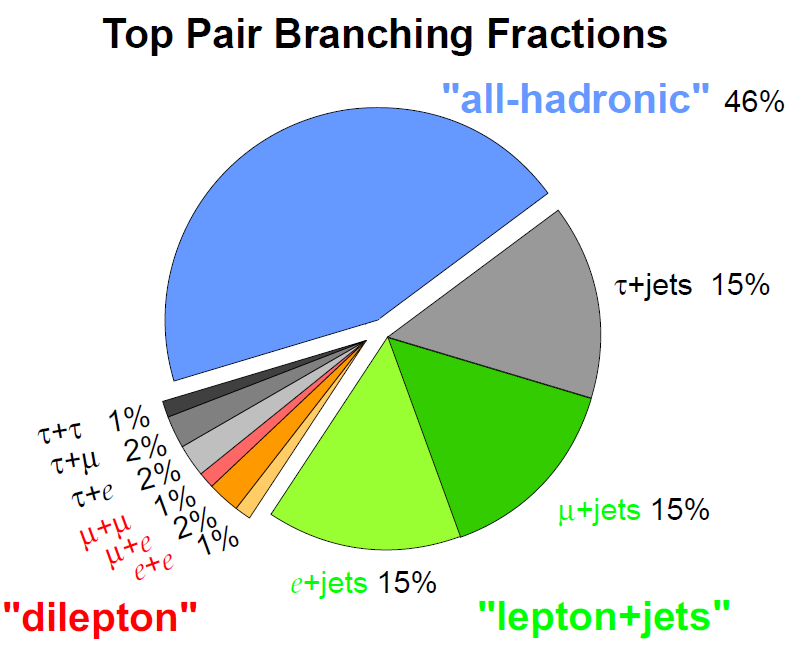
\includegraphics[width=0.50\textwidth]{fig_TopQuark/Top_Pair_Branching_Fractions.png}
    \end{tabular}
    \caption{A schematic classifying \ttbar decay modes (Left), and chart showing the relative branching fractions (Right)~\cite{d0_diagrams}
            }
    \label{Top_Pair_Decay_Channels}
  \end{center}
\end{figure}

Furthermore, $\tau$ can decay either hadronically or leptonically via a virtual $W$-boson.
For lepton decays of $\tau \rightarrow \ell \bar{\nu_\ell} \nu_\tau$, the $\tau$ decays into a lepton, an anti-neutrino of the same lepton flavor, and a $\tau$ flavor neutrino.
The lepton branching fractions of $\tau$ decays are \sim$(17.82 \pm 0.04 ) \%$ for $\ell = e$ and $(17.39 \pm 0.04) \%$ for $\ell = \mu$~\cite{bib:PDG}.
Including $\tau$ decays, the \ttbar dileptonic final state branching fraction is \sim$6.42 \% = $ \sim$4.55 \% \; (\text{Prompt}) + $ \sim$1.87 \% \; (\text{Via Tau})$.
The \ttbar dileptonic final state is further categorized into three channels: \ee, \emu, and \mumu, with the combination of the three channels, denoted $\ell \bar{\ell}$.

\section{Top Quark Spin in \ensuremath{\mathrm{t\bar{t}}} Production and Top Decay}
\label{Top_Quark_Spin_in_ttbar_Production_and_Top_Decay}
In general, hadronization of quarks dilutes their spin information.
Moreover, the spins of quarks can be depolarized by processes such as gluon radiation, causing spin decorrelation.
For the top quark however, it has already been mentioned that the full decay width $\Gamma_t = 1.42 \substack{+0.19 \\ -0.15} \; \si{\GeV}$~\cite{bib:PDG} is larger than the QCD hadronization scale ($\Lambda_{QCD} \simeq \SI{0.38}{\GeV}$~\cite{Groote_1998}) and much larger than the spin decorrelation scale ($\Lambda_{QCD}^2/m_t \sim \SI{0.08}{\MeV}$~\cite{Stelzer_1996}).
Thus, not only does a top quark decay before hadronizing to form bound states but also its spin properties are transferred, without dilution, to its decay products and that information is observable in their angular kinematic distributions.
These properties make top quarks unique in the quark sector, as top quark measurements are the only opportunity to study the spin properties of free quarks.

For the spin quantization axes, we consider the top quark helicity basis ($\hat{k}, \hat{n}, \hat{r}$) in the zero momentum frame (ZMF) of the \ttbar system.
In this reference frame, the helicity axis $\hat{k}$, is defined as the direction of the top quark.
The axis $\hat{n}$ is transverse to the production plane made by $\hat{k}$ direction of the incoming parton $\hat{p}$, i.e. the direction of the proton beam $\hat{z}$, and the axis $\hat{r}$ is orthogonal to the other two axes, forming a right-handed coordinate system:
\begin{linenomath*}
\begin{align}
\begin{array}{c}
\hat{n}=\frac{\operatorname{sign}(\cos \Theta)}{\sin \Theta}(\hat{p} \times \hat{k}) \\
\hat{r}=\frac{\operatorname{sign}(\cos \Theta)}{\sin \Theta}(\hat{p} - \hat{k}\cos \Theta)
\end{array}
\label{helcity_basis}
\end{align}
\end{linenomath*}
where $\Theta$ is the top quark scattering angle and $\operatorname{sign}(\cos \Theta)$ defines a “forward” direction for each event, the importance of which will be made explicit later, so that $\hat{n}$ and $\hat{r}$ flip signs as $\Theta$ crosses $\frac{\pi}{2}$.
The helicity basis spin quantization axes are shown in figure~\ref{helicity_basis}.
\begin{figure}[htb]
  \begin{center}
    \begin{tabular}{c}
        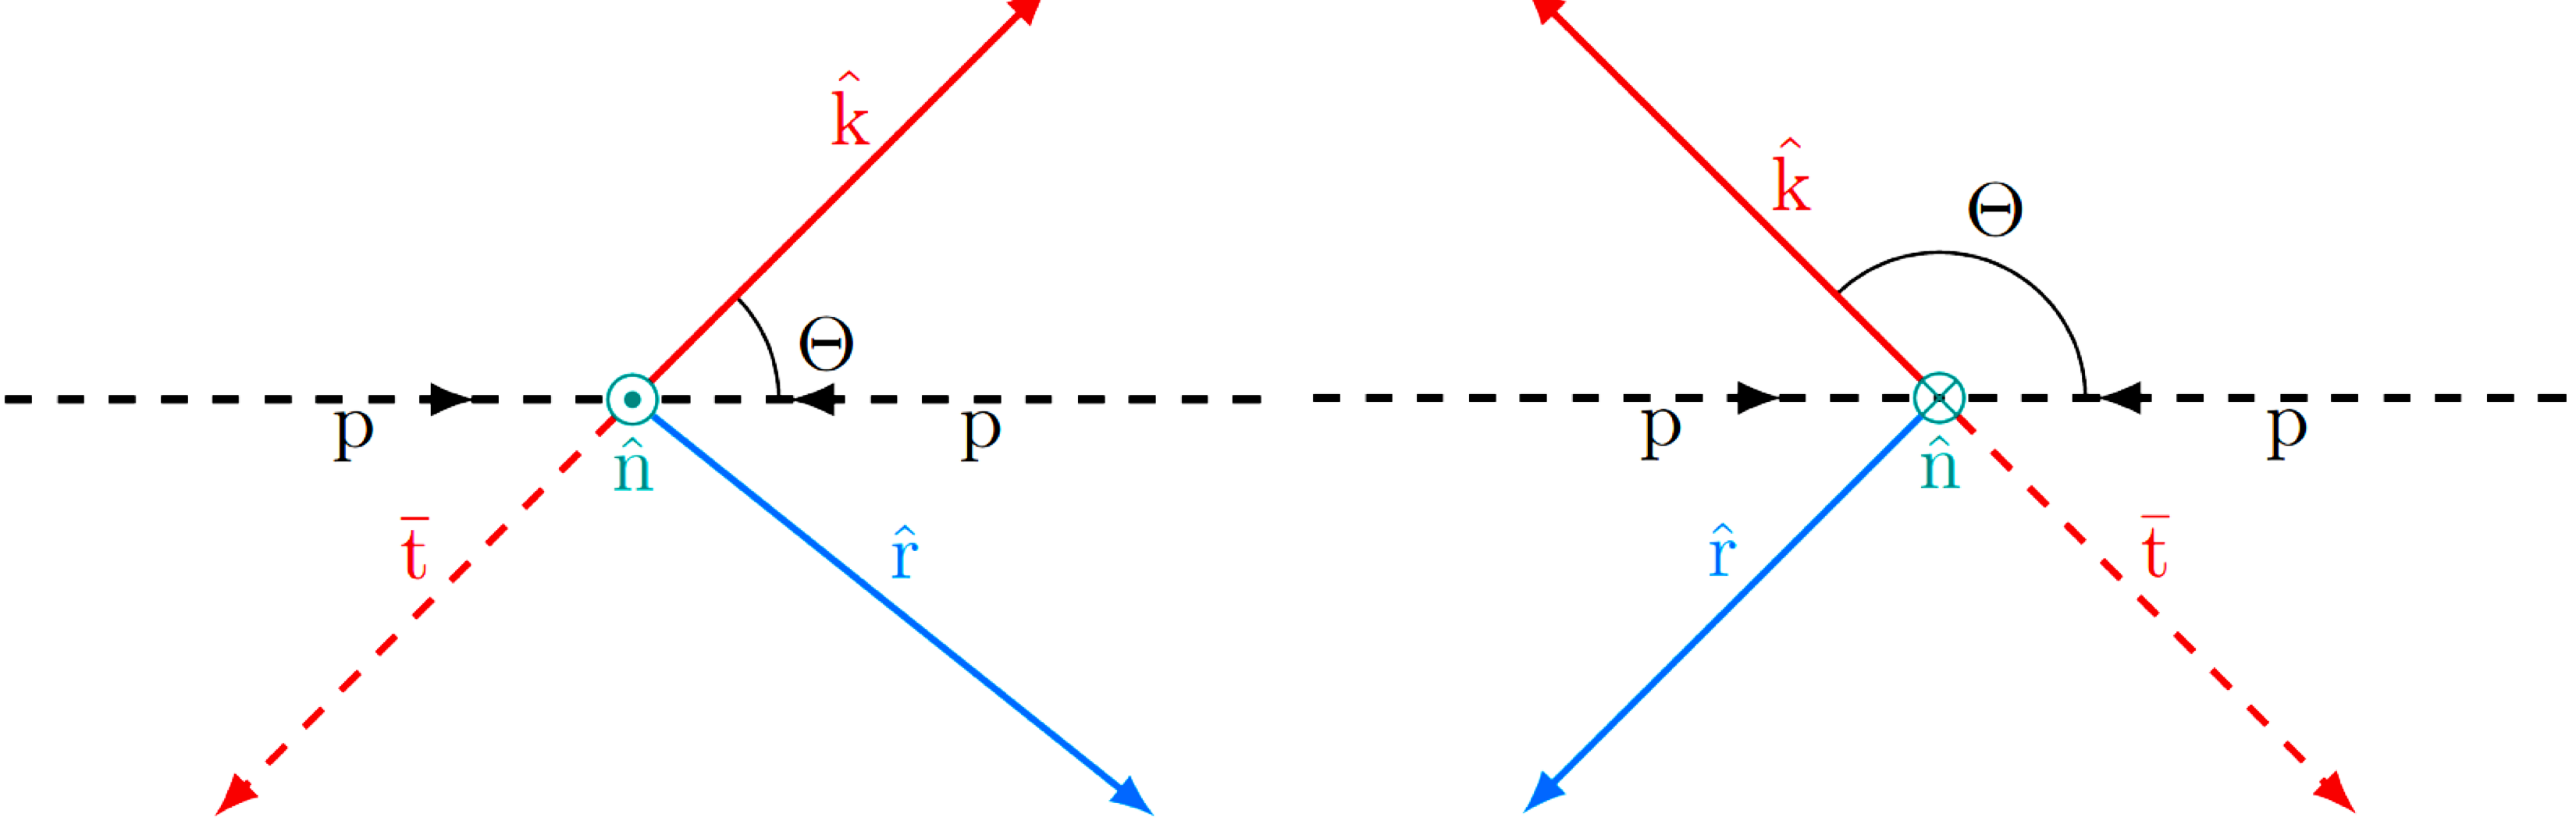
\includegraphics[width=0.99\textwidth]{fig_TopQuark/helicity_basis.png}
    \end{tabular}
    \caption{The helicity basis spin quantization axes in the \ttbar ZMF;
            $\hat{n}$ and $\hat{r}$ flip signs as $\Theta$ crosses $\frac{\pi}{2}$.
            }
    \label{helicity_basis}
  \end{center}
\end{figure}

At LO, the kinematic and spin properties of a \ttbar pair can be completely described in the \ttbar ZMF by the invariant mass $m_{\ttbar}$ and the top scattering angle $\Theta$.
Helicity is defined as spin direction projected onto the linear momentum direction, and for massive particles, helicity is reference frame dependent.
In the helicity basis of the \ttbar ZMF, squared matrix elements (see section~\ref{sec:Matrix_Element_Calculation_and_Production_Cross-section}) for the $q\bar{q}$ annihilation LO Feynman diagram in figure~\ref{ttbar_production_LO_feynman_diagrams}, separated into like-helicity ($L L, R R$) and unlike-helicity ($L R, R L$) \ttbar pairs, are~\cite{PhysRevD.53.4886}:
\begin{linenomath*}
\begin{align}
\begin{array}{c}
\sum_{L L, R R}\vert\mathcal{M}(q \bar{q} \rightarrow t \bar{t})\vert^2=8 (4 \pi \alpha_S)^2 \left(1-\beta^2\right) \sin ^2 \Theta \\
\sum_{L R, R L}\vert\mathcal{M}(q \bar{q} \rightarrow t \bar{t})\vert^2=8 (4 \pi \alpha_S)^2 \left(1+\cos ^2 \Theta\right)
\end{array}
\label{qq_matrix_elements}
\end{align}
\end{linenomath*}
where $\beta=\sqrt{1-4 m_t^2 / m_{\ttbar}^2}$ is the speed of the top quark (as a fraction of $c$) in the \ttbar ZMF and is completely determined by $m_{\ttbar}$.
In the helicity basis of the \ttbar ZMF, squared matrix elements for the $gg$ fusion LO Feynman diagram in figure~\ref{ttbar_production_LO_feynman_diagrams} separated into like-helicity ($L L, R R$) and unlike-helicity ($L R, R L$) \ttbar pairs are~\cite{PhysRevD.53.4886}:
\begin{linenomath*}
\begin{align}
\begin{array}{c}
\sum_{L L, R R}\vert\mathcal{M}(g g \rightarrow t \bar{t})\vert^2=\frac{16}{3} (4 \pi \alpha_S)^2 (\frac{7+9 \beta^2 \cos ^2 \Theta}{\left(1-\beta^2 \cos ^2 \Theta\right)^2}) \left(1-\beta^2\right)\left(1+\beta^2+\beta^2 \sin ^4 \Theta\right) \\
\sum_{L R, R L}\vert\mathcal{M}(g g \rightarrow t \bar{t})\vert^2=\frac{16}{3} (4 \pi \alpha_S)^2 (\frac{7+9 \beta^2 \cos ^2 \Theta}{\left(1-\beta^2 \cos ^2 \Theta\right)^2}) \beta^2 \sin ^2 \Theta\left(1+\cos ^2 \Theta\right).
\end{array}
\label{gg_matrix_elements}
\end{align}
\end{linenomath*}
These expressions include summation over the spins of the incoming partons, as well as summation over the colors of both the incoming and outgoing states, but factors averaging over the spins and colors have not been included.

Equations~\ref{qq_matrix_elements} indicate that in the high energy limit ($\beta \rightarrow 1$), the production of like-helicity \ttbar pairs by $q\bar{q}$ annihilation is suppressed.
Equations~\ref{gg_matrix_elements} indicate that in the high energy limit ($\beta \rightarrow 1$), the production of like-helicity \ttbar pairs by $gg$ fusion is also suppressed, but additionally at low energies $\beta << 1$, production of unlike-helicity \ttbar pairs is suppressed relative to the production of like-helicity pairs by a factor ($\beta^2$).
Figure~\ref{LHC_ttbar_helicity_differential} shows the breakdown of the total \ttbar cross-section into like-helicity and unlike-helicity pairs as a function of $m_{\ttbar}$ using the helicity basis for the $\sqrt{s}=\SI{14}{\TeV}$ LHC.
Near threshold, the dominant spin states of the \ttbar system are ${}^{1}S_{0}$ for like-helicity \ttbar pairs from $gg$ fusion and ${}^{3}S_1$ for unlike-helicity \ttbar pairs from $q\bar{q}$ annihilation:
\begin{linenomath*}
\begin{align}
{}^{1}S_{0} :
\begin{cases}
\frac{1}{\sqrt{2}}[\vert \uparrow \downarrow \rangle - \vert \downarrow \uparrow \rangle]
\end{cases}
{}^{3}S_1 :
\begin{cases} 
\vert \uparrow \uparrow \rangle \\
\frac{1}{\sqrt{2}}[\vert \uparrow \downarrow \rangle + \vert \downarrow \uparrow \rangle] \\
\vert \downarrow \downarrow \rangle 
\end{cases}
\end{align}
\end{linenomath*}
where the first (second) arrow of $\vert \uparrow \downarrow \rangle$ refers to the spin state of the top quark (anti-quark) along spin quantization axis $\hat{i}$ ($\hat{j}$).
It will be demonstrated in section~\ref{Top_Quark_Polarizations_and_ttbar_Spin_Correlations} that the different parton production processes and helicity combinations manifest themselves in the \ttbar final state particle angular kinematic distributions.
\begin{figure}[htb]
  \begin{center}
    \begin{tabular}{c}
        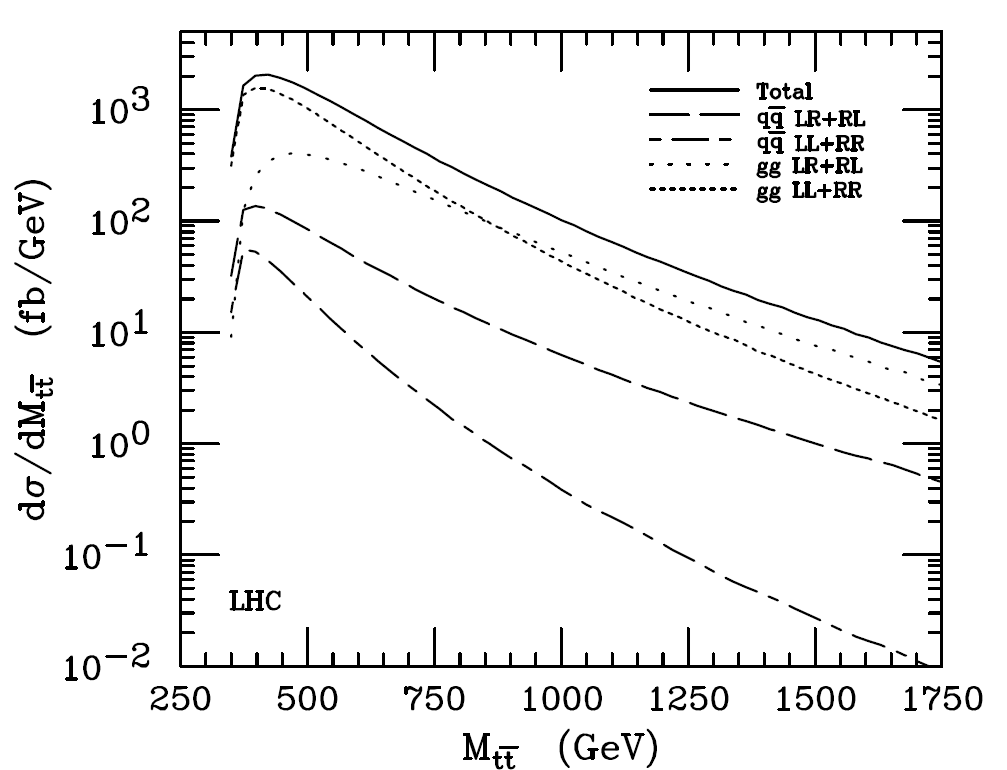
\includegraphics[width=0.7\textwidth]{fig_TopQuark/LHC_ttbar_helicity_differential.png}
    \end{tabular}
    \caption{Differential cross section for \ttbar production as a function of $m_{\ttbar}$, for the $\sqrt{s}=\SI{14}{\TeV}$ LHC, decomposed into $L L + R R$ and $L R + R L$ helicities in the zero momentum frame of the \ttbar pair for both $q\bar{q}$ and $gg$ components using the helicity basis~\cite{PhysRevD.53.4886}.
            }
    \label{LHC_ttbar_helicity_differential}
  \end{center}
\end{figure}

The differential decay rate of top quark daughter or granddaughter particle $x$, for an ensemble of polarized top quarks at rest with polarization $0 \leq \vect{P} \leq 1$, can be parameterized~\cite{BRANDENBURG2002235} as:
\begin{linenomath*}
\begin{align}
\frac{1}{\Gamma} \frac{d \Gamma}{d\left(\cos \theta_x\right)}=\frac{1}{2}[1+ \vert \vect{P} \vert \kappa_x \cos \theta_x]
\end{align}
\end{linenomath*}
where $\theta_x$ is the angle between $\vect{P}$ and the momentum direction of $x$ in the top quark ZMF and $\kappa_x$ is the top spin analyzing power of particle $x$, denoting what fraction of the top polarization information gets transferred from the top to its daughter or granddaughter particle $x$.
The top spin analyzing power at NLO is shown for the various daughter and granddaughter particles in table~\ref{spin_analyzing_power_NLO}.
\begin{table}[htb]
\begin{center}
\begin{tabular}{lr}
\multicolumn{2}{c}{ Top Spin Analyzing Power at NLO } \\
\hline$\kappa_b$ & $-0.39$ \\
$\kappa_{W^{+}}$ & $0.39$ \\
$\boldsymbol{\kappa}_{\ell}$ & $\mathbf{0.998}$ \\
$\kappa_{\bar{d}, \bar{s}}$ & $0.93$ \\
$\kappa_{u, c}$ & $-0.31$
\end{tabular}
\caption{The top spin analyzing power at NLO for the various daughter and granddaughter decay particles of the top quark~\cite{BRANDENBURG2002235}.
         }
\label{spin_analyzing_power_NLO}
\end{center}
\end{table}
For charged lepton granddaughters of top quarks, the top spin analyzing power ($\kappa_\ell$) is close to unity, and when combined with the experimental advantages that charged leptons can be triggered on efficiently and reconstructed precisely, it is concluded that the leptonic decay mode is the optimal proxy for studies of top quark spin properties.

\section{Top Quark Polarizations and \ensuremath{\mathrm{t\bar{t}}} Spin Correlations}
\label{Top_Quark_Polarizations_and_ttbar_Spin_Correlations}
Top quarks and anti-quarks, produced in \ttbar pairs at hadron colliders via the strong interaction, are not polarized at LO due to the parity conserving nature of QCD (longitudinal polarization) and approximate T-invariance of QCD (transverse polarization).
However, as was shown in the previous section, the spins of top quarks produced in \ttbar pairs are strongly correlated with spins of anti-top quarks, with dependence on $m_{\ttbar}$, $\Theta$, and choice of spin quantization axes. 
The squared matrix element for the \ttbar production and decay can be written as~\cite{Bernreuther}:
\begin{linenomath*}
\begin{align}
\begin{array}{c}
\vert\mathcal{M}(gg/q\bar{q} \to \ttbar \to (\bar{\ell} \nu_\ell b)(\ell^\prime \bar{\nu_{\ell^\prime}} \bar{b}) )\vert^2 \sim Tr[\rho R \bar{\rho}]
\end{array}
\label{ttbar_squared_matrix_element}
\end{align}
\end{linenomath*}
where $R$ is the spin density matrix related to on-shell \ttbar production and $\rho$ is the decay density matrix.
The production spin density matrix $R$ can be decomposed in the spin spaces of $t$ and $\bar{t}$ using a basis of Pauli matrices~\cite{Bernreuther}:
\begin{linenomath*}
\begin{align}
R^I \propto \tilde{A} \mathbbm{1} \otimes  \mathbbm{1} + \tilde{B}_i^+ \sigma^i \otimes \mathbbm{1} + \tilde{B}_j^- \mathbbm{1} \otimes \sigma^j + \tilde{C}_{ij} \sigma^i \otimes \sigma^j
\label{spin_density_matrix_decomposition}
\end{align}
\end{linenomath*}
where intial state $I = gg / q\bar{q}$ at fixed energy and top direction, $\tilde{A}$ determines the differential cross section for \ttbar production, $\mathbbm{1}$ is the $2\times2$ identity matrix, $\sigma^{i(j)}$ are the Pauli matrices, $\tilde{B}^\pm$ are 3-vectors that characterize the top quark ($+$) and anti-quark ($-$) polarizations along each of the spin quantization axes, and $\tilde{C}$ is a $3\times3$ matrix that characterizes the correlations between the top quark and anti-quark spins along each pair of spin quantization axes.
$\tilde{B}_i^\pm$ and $ \tilde{C}_{ij} $ can be further decomposed using the \ttbar ZMF helicity basis $\{\hat{k},\hat{n},\hat{r}\}$~\cite{Bernreuther}:
\begin{linenomath*}
\begin{align}
\begin{array}{l}
\tilde{B}_i^\pm =  b_k^\pm \hat{k_i} + b_n^\pm \hat{n_i} + b_r^\pm \hat{r_i} \\
\tilde{C}_{ij}  =  c_{kk} \hat{k_i}\hat{k_j} + c_{nn} \hat{n_i}\hat{n_j} + c_{rr} \hat{r_i}\hat{r_j} \\ 
\;\;\;\;\; + \; c_{rk} (\hat{r_i}\hat{k_j} + \hat{k_i}\hat{r_j}) +  c_{kn} (\hat{k_i}\hat{n_j} + \hat{n_i}\hat{k_j})  +  c_{nr} (\hat{n_i}\hat{r_j} + \hat{r_i}\hat{n_j}) \\
\;\;\;\;\; + \; c_{n} (\hat{r_i}\hat{k_j} - \hat{k_i}\hat{r_j}) +  c_{r} (\hat{k_i}\hat{n_j} - \hat{n_i}\hat{k_j})  +  c_{k} (\hat{n_i}\hat{r_j} - \hat{r_i}\hat{n_j})
\end{array}
\label{spin_density_matrix_decomposition_expansion}
\end{align}
\end{linenomath*}
where the coefficients $b^\pm$ and $c$ are functions of $m_{\ttbar}$ and $\cos \Theta$.
The helicity basis is chosen because of its stability with regard to reconstruction errors and the spin correlations are strong using this basis.
By construction, the coefficient functions $b^\pm$ and $c$ have definite properties with respect to discrete symmetries $P$, $CP$, $T_N$ (naive time-reversal symmetry at tree-level), and identical particle exchange ($Bose$), and as a result, these coefficients can help distinguish NP effects with SMEFT~\cite{Bernreuther}.
The $P$, $CP$, and $T$ invariance of QCD forces many of these coefficients to be zero before considering electroweak and higher-order QCD loop corrections.
The Bose symmetry of $I = gg$ implies $R^{gg}(\hat{k},\hat{p}) = R^{gg}(-\hat{k},\hat{p})$; hence the importance of $\operatorname{sign}(\cos \Theta)$ in the definition of $\{\hat{k},\hat{n},\hat{r}\}$ (see equation~\ref{helcity_basis}), to allow non-zero coefficients when the parton production process is $gg$ fusion.
A summary of transformation properties of the coefficient functions with respect to $P$, $CP$, $T_N$, and $Bose$ ($I = gg$ only) symmetries~\cite{Bernreuther} is shown in table~\ref{coefficient_function_symmetries}, 
\begin{table}[htb]
\begin{center}
\begin{math}
\begin{array}{|c|c|c|c|c|c|}
\hline
& \mathrm{CP} & \mathrm{P} & \mathrm{T}_{\mathrm{N}} & \mathrm{CPT}_{\mathrm{N}} & \text { Bose } \\
\hline 
A^I & A^I & A^I & A^I & A^I & A^{g g} \\
b_r^{I \pm} & b_r^{I \mp} & -b_r^{I \pm} & b_r^{I \pm} & b_r^{I \mp} & b_r^{g g \pm} \\
b_k^{I \pm} & b_k^{I \mp} & -b_k^{I \pm} & b_k^{I \pm} & b_k^{I \mp} & b_k^{g g \pm} \\
b_n^{I \pm} & b_n^{I \mp} & b_n^{I \pm} & -b_n^{I \pm} & -b_n^{I \mp} & b_n^{g g \pm} \\
c_{r r}^I & c_{r r}^I & c_{r r}^I & c_{r r}^I & c_{r r}^I & c_{r r}^{g g} \\
c_{k k}^I & c_{k k}^I & c_{k k}^I & c_{k k}^I & c_{k k}^I & c_{k k}^{g g} \\
c_{n n}^I & c_{n n}^I & c_{n n}^I & c_{n n}^I & c_{n n}^I & c_{n n}^{g g} \\
c_{r k}^I & c_{r k}^I & c_{r k}^I & c_{r k}^I & c_{r k}^I & c_{r k}^{g g} \\
c_{r n}^I & c_{r n}^I & -c_{r n}^I & -c_{r n}^I & -c_{r n}^I & c_{r n}^{g g} \\
c_{k n}^I & c_{k n}^I & -c_{k n}^I & -c_{k n}^I & -c_{k n}^I & c_{k n}^{g g} \\
c_r^I & -c_r^I & -c_r^I & -c_r^I & c_r^I & c_r^{g g} \\
c_k^I & -c_k^I & -c_k^I & -c_k^I & c_k^I & c_k^{g g} \\
c_n^I & -c_n^I & c_n^I & c_n^I & -c_n^I & c_n^{g g} \\
\hline
\end{array}
\end{math}
\caption{Transformation properties of the coefficient functions with respect to CP, P, and $\mathrm{T_N}$ symmetries for $I = gg, q\bar{q}$~\cite{Bernreuther}. 
        In the last column, all the coefficients of the initial state $I = gg$ are even under Bose symmetry because of the $\operatorname{sign}(\cos \Theta)$ factor in the definition of $\{\hat{k},\hat{n},\hat{r}\}$ (see equation~\ref{helcity_basis}).
        }
\label{coefficient_function_symmetries}
\end{center}
\end{table}

As has been already mentioned, top quark spins cannot be measured directly but can be traced in the differential angular distributions of their charged lepton granddaughters.
For \ttbar dileptonic events, the normalized fourfold angular cross-section~\cite{Bernreuther} for the two leptons is:
\begin{linenomath*}
\begin{align}
\frac{1}{\sigma} \frac{d \sigma}{d \Omega_1 d \Omega_2}=\frac{1}{(4 \pi)^2}\left(1+\vec{B}_1 \cdot \hat{\bar{\ell}}_1+\vec{B}_2 \cdot \hat{\ell}_2-\hat{\bar{\ell}}_1 \cdot \matr{C} \cdot \hat{\ell}_2\right)
\label{fourfold_angular_distribution}
\end{align}
\end{linenomath*}
where $\hat{\bar{\ell}}_1$ ($\hat{\ell}_2$) is the charged lepton direction in the ZMF of its grandmother top quark (anti-quark).
$\vec{B}_{1(2)}$ are 3-vectors sensitive to $\tilde{B}^\pm$, and $\matr{C}$ is a $3\times3$ matrix sensitive to $\tilde{C}$.
Each coefficient probes a single coefficient function:
\begin{itemize}
\item The top (anti-top) polarization coefficients are $B_1^{i}$ ($B_2^{j}$), with respect to spin quantization axis $\hat{i}$ ($\hat{j}$), and are sensitive to coefficient functions $b^+_i$ ($b^-_j$).
\item The diagonal spin correlation coefficients are $C_{ii}$, with respect to spin quantization axis $\hat{i}$, and are sensitive to $c_{ii}$.
\item The cross spin correlation coefficients are $C_{ij}$ and $C_{ji}$,  for each pair of spin quantization axes $\hat{i}$ and $\hat{j}$, with the sums and differences $C_{ij} \pm C_{ji}$ sensitive to $c_{ij}$ and $c_{i}$~\ref{spin_density_matrix_decomposition_expansion}.
\end{itemize}
Unlike the coefficient functions of $\tilde{B}^\pm$ and $\tilde{C}$, the coefficients of $\vec{B}_{1(2)}$ and $\matr{C}$ are directly observable final state variables.
A summary of the polarization and spin correlation coefficients, which coefficient functions they probe, and which contributions in the differential parton cross-sections the coefficients are sensitive to, is summarized in table~\ref{coefficients_sensitive}.
\begin{table}[htb]
\begin{center}
\begin{math}
\begin{array}{|c|c|c|}
\hline 
\text { Coefficients } & \text { Coefficient Functions } & \text { Contributions } \\
\hline 
C_{nn} & c_{n n}^I & \text { P-, CP-even } \\
C_{rr} & c_{r r}^I & \text { P-, CP-even } \\
C_{kk} & c_{k k}^I & \text { P-, CP-even } \\
C_{rk}+C_{kr} & c_{r k}^I & \text { P-, CP-even } \\
C_{nr}+C_{rn} & c_{r n}^I & \text { P-odd, CP-even, absorptive } \\
C_{nk}+C_{kn} & c_{k n}^I & \text { P-odd, CP-even, absorptive } \\
C_{rk}-C_{kr} & c_n^I & \text { P-even, CP-odd, absorptive } \\
C_{nr}-C_{rn} & c_k^I & \text { P-odd, CP-odd } \\
C_{nk}-C_{kn} & -c_r^I & \text { P-odd, CP-odd } \\
B_1^{n}+B_2^{n} & b_n^{I+}+b_n^{I-} & \text { P-, CP-even, absorptive } \\
B_1^{n}-B_2^{n} & b_n^{I+}-b_n^{I-} & \text { P-even, CP-odd } \\
B_1^{r}+B_2^{r} & b_r^{I+}+b_r^{I-} & \text { P-odd, CP-even } \\
B_1^{r}-B_2^{r} & b_r^{I+}-b_r^{I-} & \text { P-odd, CP-odd, absorptive } \\
B_1^{k}+B_2^{k} & b_k^{I+}+b_k^{I-} & \text { P-odd,CP-even } \\
B_1^{k}-B_2^{k} & b_k^{I+}-b_k^{I-} & \text { P-odd, CP-odd, absorptive } \\
\hline
\end{array}
\end{math}
\caption{A summary of the polarization and spin correlation coefficients, which coefficient functions they probe, and which contributions in the differential parton cross-sections the coefficients are sensitive to~\cite{Bernreuther}. 
        }
\label{coefficients_sensitive}
\end{center}
\end{table}

Integrating out the azimuthal angles of the normalized fourfold angular cross-section~\ref{fourfold_angular_distribution} yields the normalized polar angle double cross-section,
\begin{linenomath*}
\begin{gather}
\label{double_angular_distribution}
\frac{1}{\sigma} \frac{d \sigma}{d \cos \theta_1^i d \cos \theta_2^j}=\frac{1}{4}\left(1+B_1^{i} \cos \theta_1^i+B_2^{j} \cos \theta_2^j-C_{ij} \cos \theta_1^i \cos \theta_2^j\right), \quad \text{where} \\
\label{Polarizations_and_Spin_Correlations}
\begin{array}{c}
B_1^{i} = P_{i}\kappa_\ell,\\
B_2^{j} = -\bar{P}_{j}\kappa_\ell,\\
C_{ij}=\kappa_{\ell}^2 \frac{\sigma(\uparrow \uparrow)+\sigma(\downarrow \downarrow)-\sigma(\uparrow \downarrow)-\sigma(\downarrow \uparrow)}{\sigma(\uparrow \uparrow)+\sigma(\downarrow \downarrow)+\sigma(\uparrow \downarrow)+\sigma(\downarrow \uparrow)}
\end{array}
\end{gather}
\end{linenomath*}
with $P_{i} = \langle 2 \vect{S_t} \cdot \hat{i} \rangle$, $\bar{P}_{j} = \langle 2 \vect{S_{\bar{t}}} \cdot \hat{j} \rangle$, and the first (second) arrow of $\sigma(\uparrow \downarrow)$ referring to the spin state of the top quark (anti-quark) along spin quantization axis $\hat{i}$ ($\hat{j}$).
The quantity $\cos \theta_1^k = \hat{\bar{\ell}}_1 \cdot \hat{k}$, as an example, can be calculated by taking the dot product of the charged lepton direction in its grandfather top quark's ZMF with the $\hat{k}$ helicity basis spin quantization axis in the \ttbar ZMF and can be demonstrated to be Lorentz invariant.

From equation~\ref{double_angular_distribution}, it can be derived that the single-differential cross-sections are given by:
\begin{linenomath*}
\begin{align}
\frac{1}{\sigma} \frac{d \sigma}{d \cos \theta_{1(2)}^i} & =\frac{1}{2}\left(1+B_{1(2)}^{i} \cos \theta_{1(2)}^i\right),
\label{single_angular_distribution_polar}
\end{align}
\begin{align}
\frac{1}{\sigma} \frac{d \sigma}{d \cos \theta_1^i \cos \theta_2^i} & =\frac{1}{2}\left(1 - C_{ii} \cos \theta_1^i \cos \theta_2^i\right) \log \left(\frac{1}{\left \vert \cos \theta_1^i \cos \theta_2^i\right \vert}\right),
\label{single_angular_distribution_diagonal}
\end{align}
\begin{align}
\frac{1}{\sigma} \frac{\mathrm{d} \sigma}{\mathrm{d} x_{\pm}} = \frac{1}{2} \left(1-\frac{C_{ij} \pm C_{ji}}{2} {x_{\pm}} \right) \cos ^{-1} \left \vert x_{\pm} \right \vert
\label{single_angular_distribution_cross}
\end{align}
\end{linenomath*}
\begin{center}
for $\hat{i} \neq \hat{j}$ where $x_{\pm} = \cos \theta_1^i \cos \theta_2^j \pm \cos \theta_1^j \cos \theta_2^i$.
\end{center}
These single-differential cross-sections would otherwise be symmetric functions if not for the presence of the coefficient parameters.
Thus the fifteen coefficients can be extracted from the mean or asymmetry of the following single-differential cross-sections:
\begin{itemize}
\item The six top quark (anti-quark) polarization coefficients $B_{1(2)}^{i}$ using~\ref{single_angular_distribution_polar},
\item  The three diagonal spin correlation coefficients $C_{ii}$ using~\ref{single_angular_distribution_diagonal}, and
\item  Sums and differences of the six cross spin correlation coefficients $C_{ij} \pm C_{ji}$ using~\ref{single_angular_distribution_cross}.
\end{itemize}

The above decomposition is true for any subset of the full phase space, so double differential measurements of the polarization and spin correlations involve partitioning the phase space and, in each partition, repeating the procedure of measuring the relevant single-differential cross-sections and then extracting the coefficients.

\section{Previous Measurements of Top Quark Polarizations and \ensuremath{\mathrm{t\bar{t}}} Spin Correlations at the LHC}
Measurements of \ttbar spin correlations in the dilepton mode have been performed by both the Compact Muon Solenoid (CMS) and ATLAS experiments using $36$ \invfb of data taken at the LHC during 2016 at a center-of-mass collision energy of \beamenergy~\cite{arxiv.1905.08634},\cite{Sirunyan:2681777},\cite{Aaboud:2667501}.
Both experiments unfolded their results to parton-level and extrapolated to the full phase space.
Both CMS and ATLAS made indirect measurements of \ttbar spin correlations by measuring $\vert \Delta\phi_{\ell\bar{\ell}} \vert$, the difference in azimuthal angle between the two leptons in the laboratory frame, but ATLAS additionally measured $\vert \Delta\eta_{\ell\bar{\ell}} \vert$, the difference in pseudorapidity between the two leptons in the laboratory frame, and performed their $\vert \Delta\phi_{\ell\bar{\ell}} \vert$ measurements differentially as a function of \ttbar invariant mass, but only made measurements in the \emu channel.
ATLAS observed a $3.2 \sigma$ deviation from the SM in their measurement of $\vert \Delta\phi_{\ell\bar{\ell}} \vert$ remains in tension with the CMS result, but could possibly be explained by missing higher-order corrections to the top quark kinematics in Monte Carlo (MC) simulations.
